\section{Partitionnement \'etendu: \'Etablir une partition}
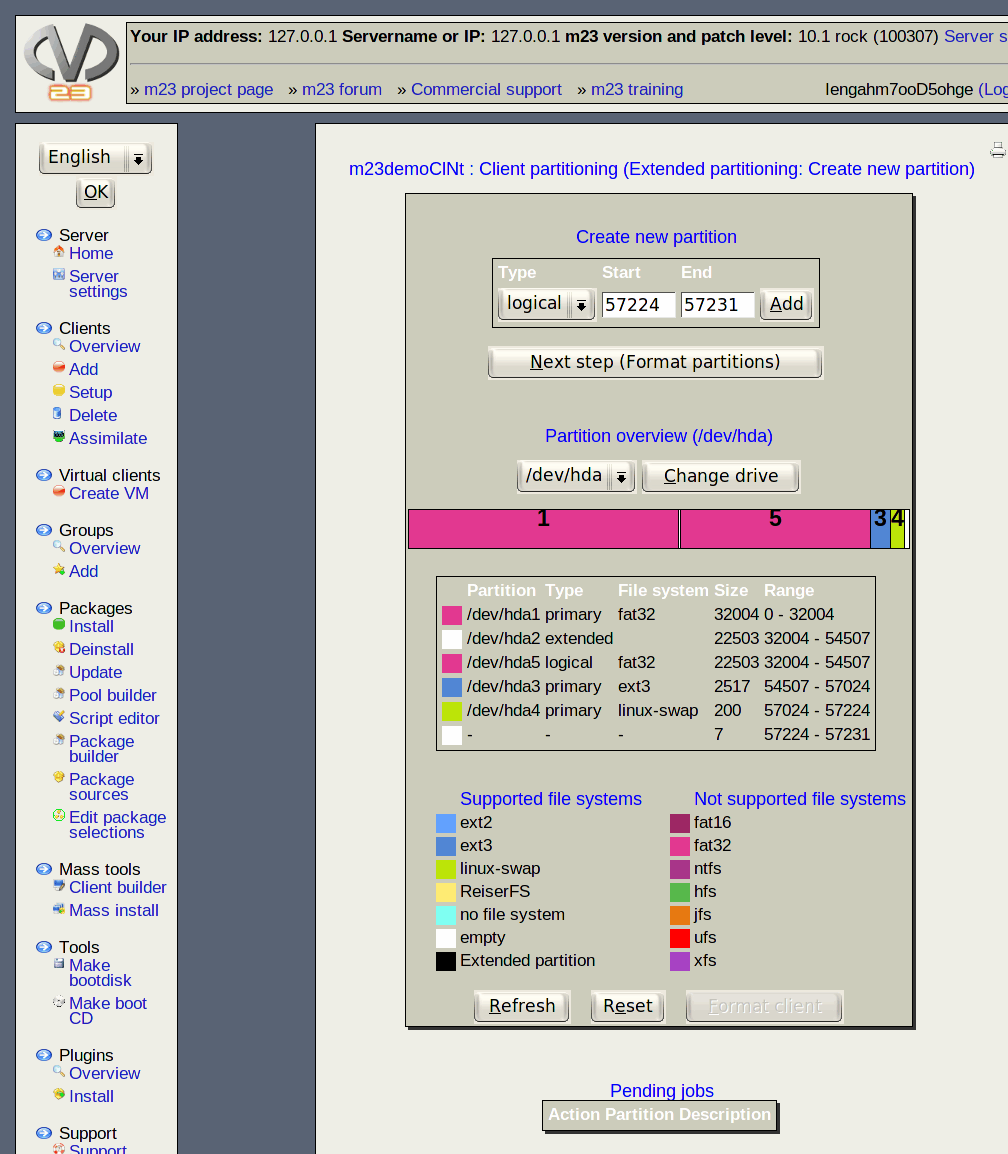
\includegraphics[scale=0.4]{/mdk/doc/manual/screenshots/fr/fdisk-extended1.png} \\
\begin{itemize}
\item Maintenant, vous pouvez \'etablir des nouvelles partitions. Vous pouvez choisir entre l'\'etablissement d'une partition primaire (primary), \'etendue (extended) ou logique (logical).\\
S\'electionnez le type de la partition et son d\'ebut et sa fin et ensuite, cliquez sur \textit{$\ll$Ajouter$\gg$}. Sous \textit{$\ll$Type$\gg$}, vous pouvez seulement choisir entre des types de partitionnement que vous pouvez \'etablir r\'eellement. Vous trouvez une information suppl\'ementaire concernant les conditions de l'\'etablissement des types de partitionnement diff\'erents en bas de la page.\\
\item Sous \textit{$\ll$Vue d'ensemble des partitions$\gg$}, vous trouvez des zones libres (marqu\'ees en blanc), dans lesquelles vous pouvez \'etablir des nouvelles partitions. Quant au point de rep\`ere pour les valeurs du d\'ebut et de la fin de vos nouvelles partitions, faites attention aux valeurs sous \textit{$\ll$Zone$\gg$}.\\
\item S'il n'y a pas assez de place pour les partitions souhait\'ees, cliquez sur le bouton \textit{$\ll$Retour$\gg$} de votre navigateur web \`a plusieures reprises jusqu'\`a ce que vous arriviez \`a la page \textit{$\ll$Effacer des partitions$\gg$}.\\
\item Quand vous avez \'etablis toutes les partitions n\'ecessaires, cliquez sur \textit{$\ll$$\gg$}.\\
\end{itemize}
\subsection{Information: Types de partitionnement}
\begin{itemize}
 \item \textbf{primaire:} Vous pouvez \'etablir un maximum de quatre partitions primaires.\\
 \item \textbf{\'etendu:} Une partition \'etendue appartient aux partitions primaires aussi. Il peut \^etre \'etabli une partition \'etendue au maximum. Au dedans d'une partition \'etendue, vous pouvez \'etablir des partitions logiques, si les quatres primaires ne vous suffiraient pas.\\
 \item \textbf{logique:} Des partitions logiques ne peuvent \^etre \'etablies que dans l'espace m\'emoire d'une partition \'etendue. Le nombre des partitions logiques n'est pas limit\'e.\\
\end{itemize}
